Aquí se presentan las vistas que contendrá la aplicación para la interacción con el usuario.

\subsection{Inicio de Sesión}

\begin{figure}[H]
    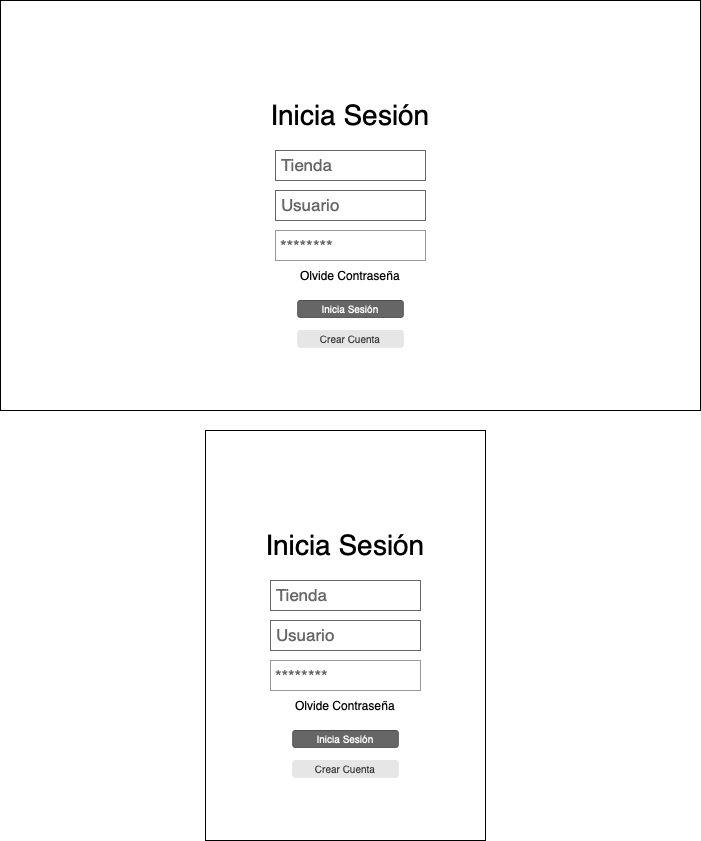
\includegraphics[width=.75\textwidth]{images/InicioSesion.png}
    \centering
    \caption{Página de inicio de sesión en web y vista de cliente Android.}
\end{figure}

La pantalla de inicio de sesión permite a los usuarios autenticarse en la aplicación ingresando sus credenciales.
En la versión web y móvil, se presenta un diseño simple con campos para usuario y contraseña, así como opciones para 
recuperar el acceso en caso de olvido.


\subsection{Crear Cuenta}

\begin{figure}[H]
    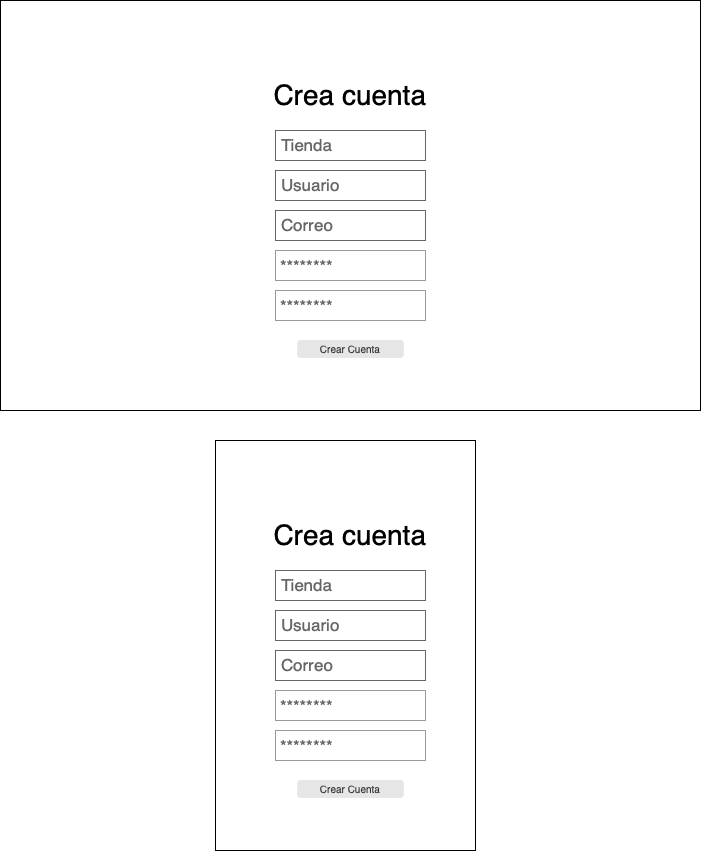
\includegraphics[width=.75\textwidth]{images/CreaCuenta.png}
    \centering
    \caption{Página para la creación de una cuenta en web y vista en cliente Android.}
\end{figure}

La interfaz de creación de cuenta permite a los nuevos usuarios registrarse proporcionando su información básica.
Se incluyen campos para nombre, correo electrónico, contraseña y nombre de tienda.

\subsection{Página de Inicio}

\begin{figure}[H]
    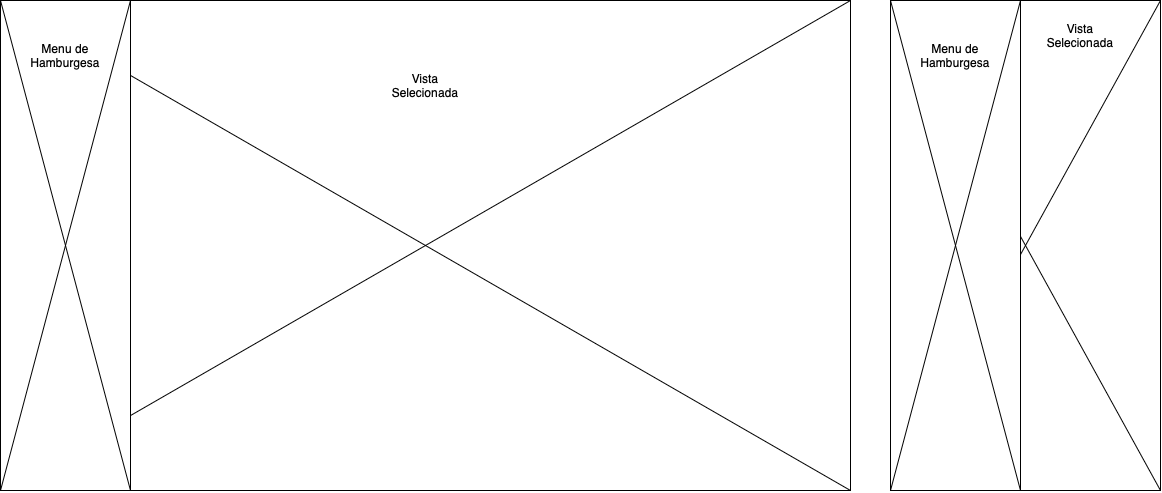
\includegraphics[width=.75\textwidth]{images/Inicio.png}
    \centering
    \caption{Página de inicio de la aplicación web y su contraparte en cliente Android.}
\end{figure}

Desde la página de inicio, los usuarios pueden navegar a las diferentes secciones de la aplicación. Contiene un menú de
hamburguesa que da acceso a las funcionalidades principales, como ventas, inventario, reportes y administración dependiendo el caso.

\subsection{Punto de Venta}

\begin{figure}[H]
    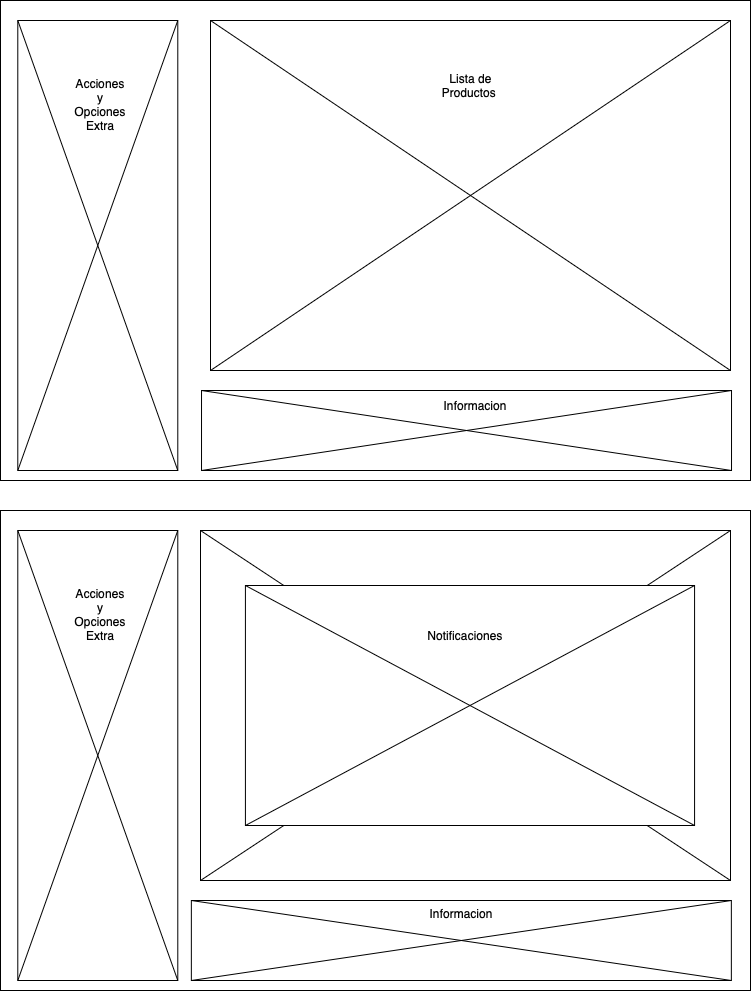
\includegraphics[width=.75\textwidth]{images/POS.png}
    \centering
    \caption{Página del punto de venta en web con notificación emergente.}
\end{figure}

La interfaz del punto de venta permite registrar ventas en tiempo real. Cuenta con un menú de hamburguesa para acceder
a funciones adicionales y una sección central donde se muestran los productos agregados al ticket.
En la parte inferior, se visualiza información relevante como cupones, descuentos y el total de la venta.
Además, pueden aparecer notificaciones emergentes para alertar al usuario sobre eventos importantes.

\subsection{Administración}

\begin{figure}[H]
    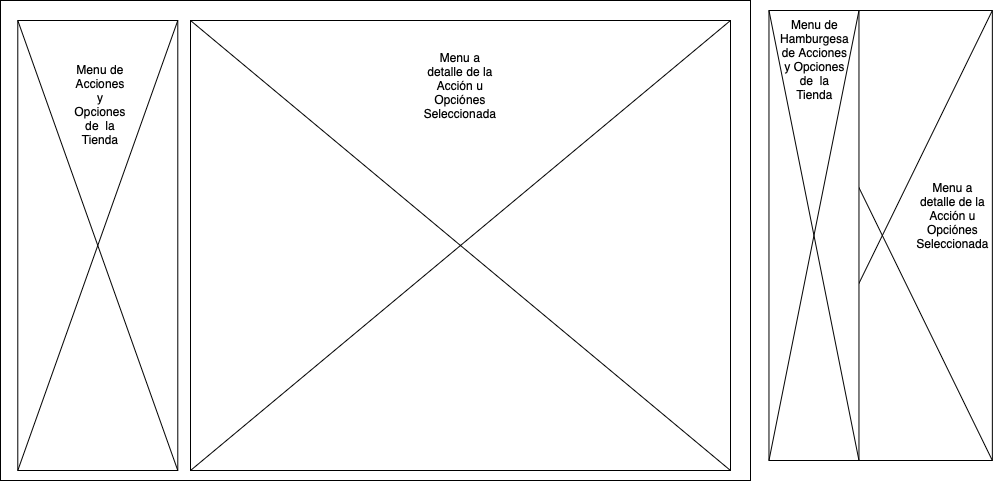
\includegraphics[width=.75\textwidth]{images/Administracion.png}
    \centering
    \caption{Página de administración de la tienda en web con su contraparte en el cliente Android.}
\end{figure}

La sección de administración permite gestionar usuarios, permisos y configuraciones generales de la tienda.
Presenta un menú de hamburguesa que facilita la navegación entre las distintas opciones de configuración.

\subsection{Manejo de Inventario}

\begin{figure}[H]
    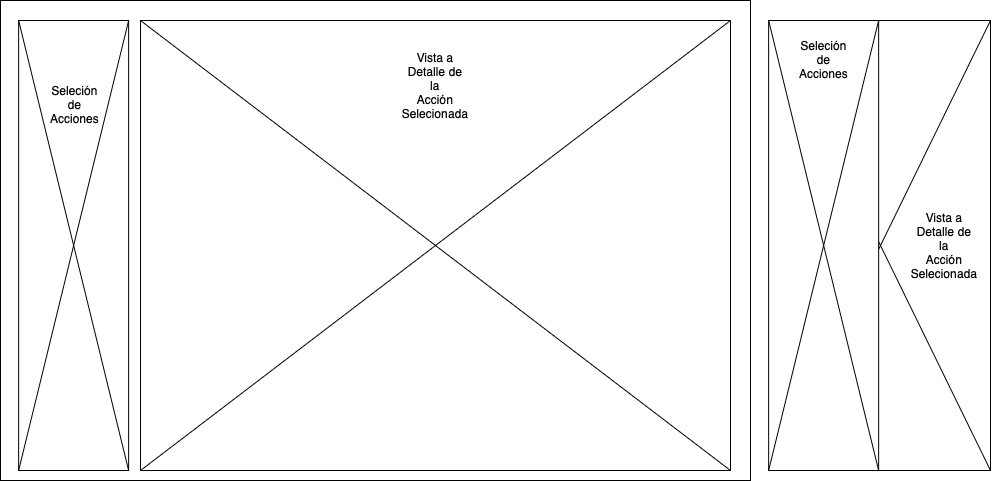
\includegraphics[width=.75\textwidth]{images/Inventario.png}
    \centering
    \caption{Página para el manejo del inventario de la tienda en web y en su vista Android.}
\end{figure}

Desde esta sección, los usuarios pueden gestionar el stock de productos, actualizar información de artículos
y realizar ajustes en el inventario. El menú de hamburguesa permite acceder a opciones como control de existencias
y gestión de proveedores.

\subsection{Análisis de Datos y Reportes}

\begin{figure}[H]
    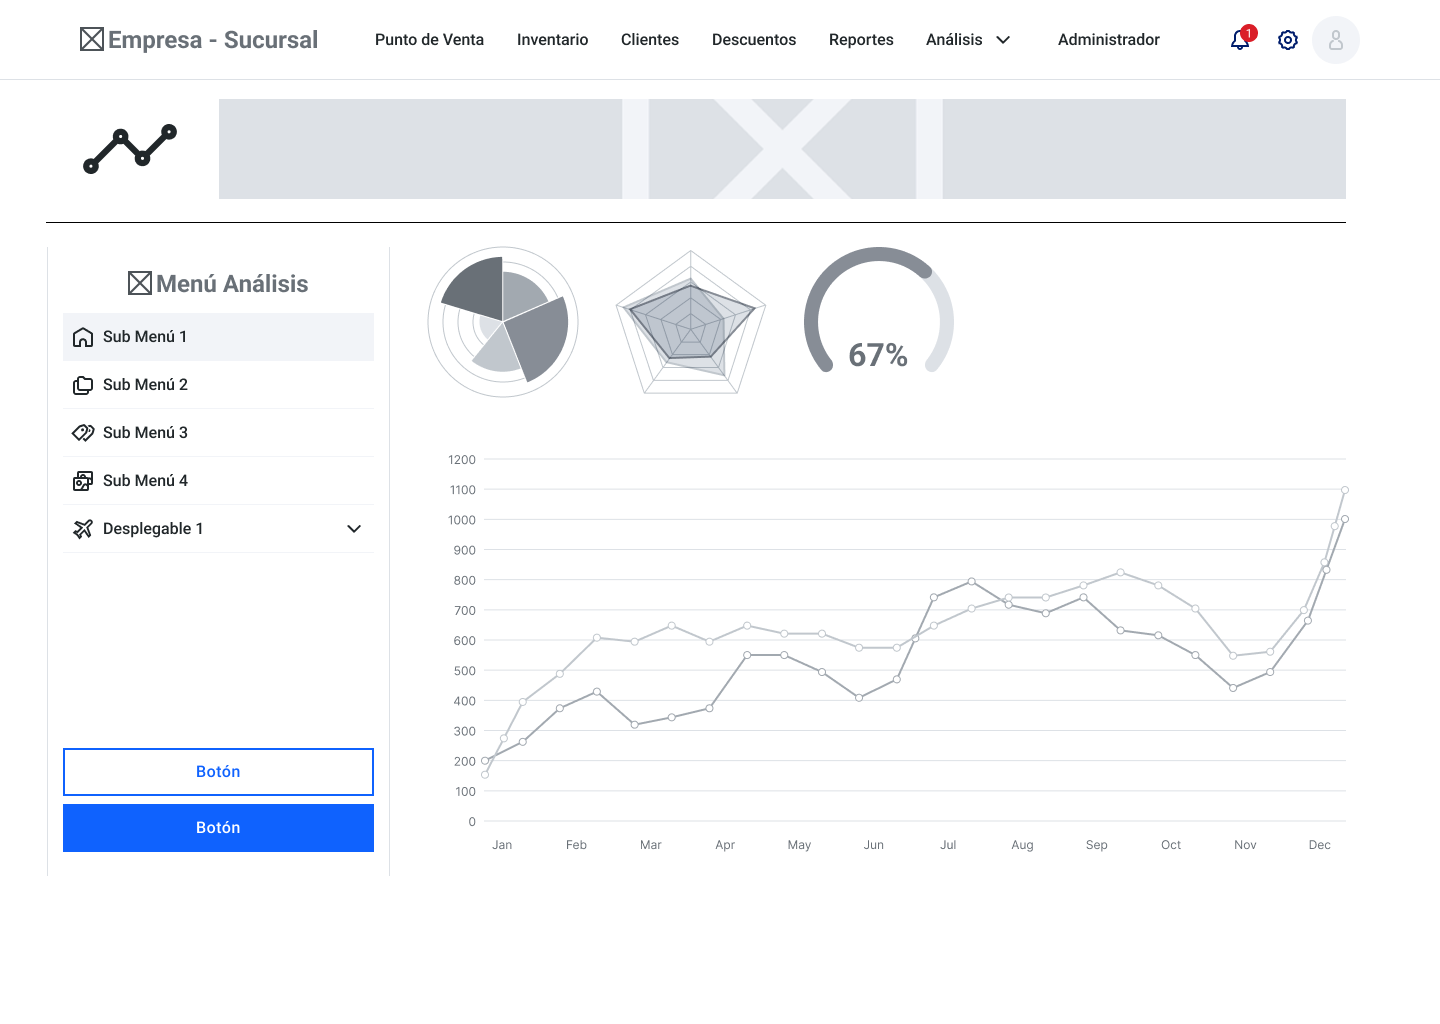
\includegraphics[width=.75\textwidth]{images/Analisis.png}
    \centering
    \caption{Página para la consulta de análisis y reportes en web y su vista correspondiente en Android.}
\end{figure}

Esta sección permite visualizar reportes y realizar análisis de datos basados en el historial de ventas e inventario.
A través del menú de hamburguesa, el usuario puede seleccionar entre generación de reportes y herramientas de predicción
de tendencias.
